\chapter{REAGENT: ENABLING INTERACTION WITH ARBITRARY WEB CONTENT}\label{chap:reagent}
\blfootnote{Portions of
  this chapter previously appeared as:
  \begin{itemize}[\indent { }]
    \item M. Peveler, J. O. Kephart, and H. Su, “Reagent: Converting ordinary webpages
into interactive software agents,” in \textit{Proc. of the 28th
Int. Joint Conf. on Artif. Intell.}. Macao,
China: Int. Joint Conf. on Artif. Intell.
Org., Aug. 2019, pp. 6560–6562.
    
    \item M. Peveler, J. O. Kephart, X. Mou, G. Clement, and H. Su, “A virtual mouse
interface for supporting multi-user interactions,” in \textit{Human-Comput.
Interact. Multimodal and Natural Interact.}, M. Kurosu, Ed. Copenhagen,
Denmark: Springer Int. Publishing, 2020, vol. 12182, pp. 497–508.
\end{itemize}}

\section{Introduction}

With the growing ubiquity of voice-activated assistants like Siri and Alexa, society is
quickly acclimating to interacting with AI as we do with our fellow humans. Now under development is
a new generation of more sophisticated assistants centered around 
cognitive spaces that are designed to help scientists, business users, and students with
cognitive tasks such as data exploration and analysis~\cite{kephart2018cognitive}, decision making~\cite{farrell2016symbiotic}, and learning languages~\cite{allen_rensselaer_2019}.

Practically all of these cognitive applications entail some sort of interaction with data that
is based on multi-modal inputs that include speech, pointing and gesture. To date, the assistants have 
supported such interactions by reading data from a database and displaying it in the form of tables or 
plots through web pages that are specially instrumented to capture pointing events. A stream of utterances 
is converted into a text stream by a speech-to-text engine and combined with the stream of pointing events 
to derive user intent, i.e. a parameterized command that is then executed by orchestrating one or more services 
and rendering the output on a display and optionally as synthesized speech played through a speaker. A 
major bottleneck in the creation of such cognitive assistants is that creating specially-instrumented web 
pages is labor-intensive. Unless this bottleneck can be removed, it seems unlikely that multi-modal cognitive
assistants will become anywhere near as pervasive as the present generation of less-sophisticated bots.

In this paper, we describe \textit{Reagent}, a novel technology that reduces the above-mentioned bottleneck by
readily converting ordinary non-instrumented webpages containing structured data into
software agents with which one can interact naturally, via a combination of speech and
pointing. \textit{Reagent} combines streams of semantically-meaningful mouse events with
speech transcriptions to derive and execute parameterized commands that represent user
requests to visualize, extract, query, sort, filter, analyze, or otherwise manipulate data
displayed on webpages. Command execution entails displaying the requested information in the
original webpage or in a dynamically-constructed one, as well as playing synthesized speech.
\textit{Reagent} automatically infers mappings from event labels to human-friendly terminology,
or when necessary learns them actively from the user. 

\textit{Reagent} takes advantage of the fact that web pages are highly structured, plus
emerging website accessibility conventions and standards that embed
information that helps interpret elements that are displayed on a given web page. 
For example, there exists a large body of guides on accessibility for sites which include the W3C Standard
Web Content Accessibility  
Guidelines\footnote{https://www.w3.org/WAI/standards-guidelines/wcag/} or a
Voluntary Product Accessibility 
Template\footnote{https://www.section508.gov/sell/vpat}. This accessibility
is aimed at improving the experience of people with disabilities, and who might
not be able to fully see and visualize the content of page. These users rely
on things like screen readers which traverse the semantic elements of a page
and speak the contents to the user. To accomplish this, these elements utilize
hidden, non-visible attributes that help to establish semantic understanding of
content on the page (e.g. headers and links) as well as showing information on
hovering on certain elements (e.g. column headers and images). Taking column headers as an example, 
while they may often be abbreviated when displayed to the end user, the full text is often available
when the user hovers over the abbreviation, i.e. the information is embedded in the page as a hidden attribute.

The remainder of the paper is organized as follows. After discussing related prior research, we describe
Reagent and its relationship to a larger immersive systems architecture in which it is embedded. We then describe a use case illustrating
how Reagent can be used to collaboratively build an ontology from scratch, pulling information from pages as users navigate and interact with them. We then perform an experiment to assess how broadly
applicable Reagent is to web pages encountered in ordinary use, finding that it works for approximately 80\% of nearly 200 popular web pages that we surveyed.
We conclude with a summary and some thoughts about future directions for this research.

\section{Prior Work}

Work on Reagent principally concerns bringing together two discrete lines
of work. The first is prior work on building intelligent system that are
capable of combining multimodal input to generate an intent for the user,
which was covered in Section~\ref{sec:cais_prior_work}. On second
line of interest, we look at the rich research on automatic extraction of
information from webpages and the lessons learned there, especially in how
they might work with ontology building. Cimiano et
al.~\cite{cimiano_towards_2004} and Storey et 
al.~\cite{storey_ontology_2005} propose frameworks on parsing
important information from web pages, which would be then encoded into RDF
structures. Gangemi~\cite{gangemi_comparison_2013} provides a recent
overview of available technologies in this space.
However, these approaches generally focus on the use of just natural
language understanding over the entire page for key terms and relations,
and not necessarily leveraging the increasingly rich ways the data may
be shown in a page that require true DOM traversal and analysis. However,
in analysis and automatic parsing of the DOM structure, we are informed
by prior work on taking into account elements that are ``noise'' (e.g.
ads and popups) which might look well-structured, but that the user most
likely does not care about. Gupta et al.~\cite{gupta_dom-based_2003}
utilizes the full DOM-tree to determine relevance of elements.
Joshi and Liu~\cite{joshi_web_2009} utilize both DOM traversal and NLP
to determine salient details. Sun et al.~\cite{sun_dom_2011} utilize a
algorithm that considers content density within nodes. Our current work
focuses on automatic analysis of elements that rarely, if ever, appear
within this ``noisy'' data, but is important to consider as we expand
Reagent to further domains. Finally, in the realm of understanding purely
tabular data, Hackinger~\cite{hackinger_datagorri:_2018} proposes a
system similar in some regards to \textit{Reagent}, but that it requires
for any new site the human to first identify the table on the page and
to present a ``template'' on how it should be parsed, acting far less
autonomously than \textit{Reagent}. These works inform our approach
on building \textit{Reagent}, but it is important to note that our
end-goal, principally in automatic on-the-fly webpage parsing and
ontology building for use in multimodal applications, is different.

\begin{comment}
% this is a slimmed diagram of the one shown in chap 2, so ignored
\begin{figure}
    \centering
    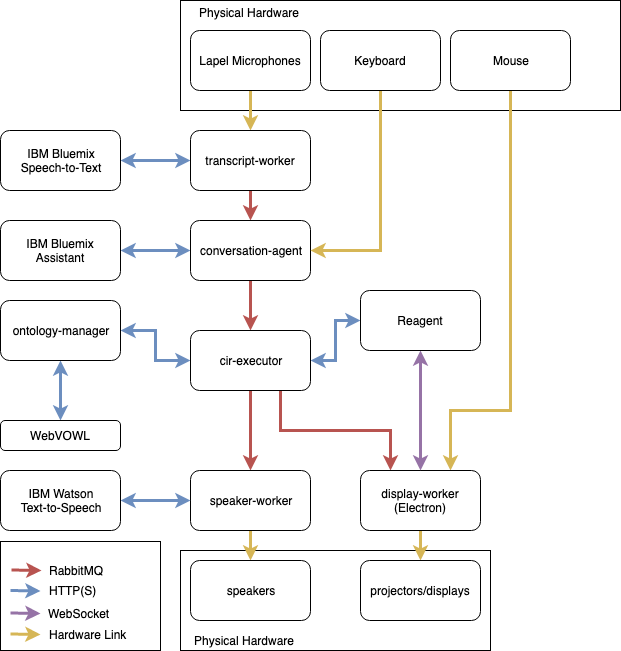
\includegraphics[width=0.45\textwidth]{chapters/03_reagent/figures/cir_diagram}
    \caption{Diagram of the Cognitive and Immersive System for Reagent}
    \label{fig:cais}
\end{figure}
\end{comment}

\section{Reagent}\label{sec:reagent}

The \textit{Reagent} system allows us a way to hook into the content that is
shown within the Electron framework discussed in Section~\ref{sec:display-worker}. The
system is broken up into two components, a central server and then the clients.
The central server is used to handle communication from the clients and the
larger CAIS architecture, as well as store information coming from the clients
for reference. This information includes the type of semantic elements exist on
the page, as well as an event stack for recorded user interactions within any
webview. Communication between the server and the clients is handled by using
websockets which facilitates real-time communication of data. To handle requests
from the CAIS, the server implements a RESTful API. The client are inserted as a
transparent layer on top of any opened webview within the system.  This
transparent layer then sets up a connection back to the central server, and then
semantically parses the page using standard DOM traversal via JavaScript
to identify key HTML structures with which a user
might interact with (e.g. a table or a plot), and uses this information to bind
appropriate event handlers to listen for user interactions, as well as for any
changes to the page's content. More specifically,

\begin{enumerate}
    \item Electron pre-loads the \textit{Reagent} system on top of the webview, and injects a websocket connection allowing it to communicate with the open webview and receive JSON-formatted events into an event buffer.
    \item Electron emits a ``DOM Ready'' event to signal that the page has finished loading, whereupon \textit{Reagent} scans the page to see if it can detect any major HTML elements it should parse and bind to (e.g. a table).
    \item \textit{Reagent} injects additional code specific to the detected HTML elements that binds event listeners to these elements as well as assigning each a UUID --- an approach that makes \textit{Reagent} readily extensible to new types of elements. (We have implemented domain-independent layers designed for general tables and for plot.ly plots, and allow for domain specific layers as well.)
    \item Next, \textit{Reagent} creates a MutationObserver\footnote{https://mzl.la/1exU78d} to watch for any changes to the page. If changes are detected, it performs any necessary re-injections and re-bindings to ensure that all relevant elements remain instrumented.
    \item Finally, \textit{Reagent} sets up a listener such that if the webview
    is closed, the client disconnects and the server is alerted.
\end{enumerate}

This sequence of events is illustrated within Figure~\ref{fig:reagent}. As an example, we discuss how the
Reagent system would bind to a HTML table and the sorts of queries it would allow for from the user. A perfect data table
is made up of some number of columns and rows where the first row, if marked with the ``th'' tag, should be viewed
as a header row with labels for the columns, and then all subsequent rows marked with the ``td``` tag as data. Reagent
scans the table, generating a list of the column names and some simple heuristics about the structure of the table. Next,
assuming that Reagent has never seen a table on this site before, it first takes all of the headers and attempts to
normalize them as appropriate for its datatype using NLTK and WordNet. Take for example, a column labelled ``won''
for a column with numeric information. Here, the system first casts the word to the present tense of the verb (``win''),
and then pluralizes on its noun form (``wins''), giving us a title more likely to be said by humans. From here, we then
use WordNet to find the variations of the word (on both its noun and verb forms) and add them as entities, if missing,
to Watson Assistant to be used for intent classification on future queries.
Finally, the system binds listeners for user interaction, which in the case of a simple table would be if a user clicks on
a cell in a table or leaves their mouse hovering over it for greater than a second. For any interaction, the client
communicates with the server, which saves a JSON object of the interaction which contains what webview it occurred in,
generated reagent UUID of the element, what row/column the cell was in, contents of the cell, and the type of interaction
it was (e.g. mouseover or click).

During the scan of HTML elements, the system is capable of taking advantage of
content added for accessibility reasons. For example, in
Fig.~\ref{fig:reagent_use_case_2}, the column for ``appearances'' was labelled ``APP''.
\textit{Reagent} identifies tags that may indicate more human-friendly terms,
such as tooltips that reveal explanatory text when a user hovers over an
element, and uses approximate text matching to infer likely associations where
possible.
In cases where the system is unable to disambiguate the semantic information, it
solicits a definition from the user. For example, with the ESPN table, the
system would ask the user (via synthesized voice) to mouse over ``the column
labeled  \textit{A}'' and state what is the attribute. Upon hearing ``Assign
attribute \textit{assists} to this column'', \textit{Reagent} stores the
mapping in a dictionary, whereupon it becomes available to any subsequently
accessed bound elements on the same webpage or host site.

\begin{figure}
\centering
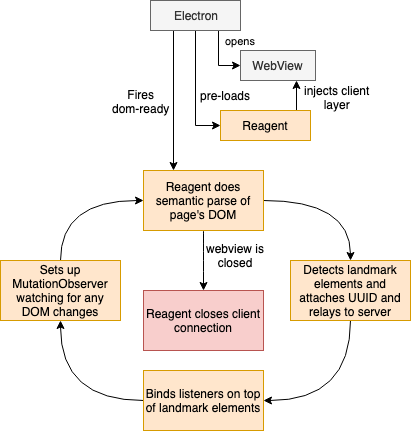
\includegraphics[width=0.45\textwidth]{chapters/03_reagent/figures/reagent.png}
\caption{Flowchart of the Reagent System.}
\label{fig:reagent}
\end{figure}

Through the transparent layer and central server described above, \textit{Reagent} enables
the executor to handle a wider range of queries that pertain to references
to the content within open webviews. At its most basic layer, the user can
query the system for the contents of the full table, what are the columns in a
table, as well as asking queries about statistics (e.g. max, min, or average)
of any given column. By capturing the interactions, it then allows the system
to handle queries that are for relative locations within the interacted with
element. For example, Figure~\ref{fig:reagent_use_case_2} illustrates the state of the
display after the user has opened an ESPN football team roster webpage and
asked the system ``Show in a new table rows where \textit{appearances} are
greater than 35.''. Equivalently, the user might have asked ``Show in a new
table rows with this column greater than this.'' while pointing to a cell
under the column `APP' with the value of 35.\footnote{For a fuller set of
capabilities that includes query, sorting, and simple analytics like averaging,
a link to a demo video is available at
\url{https://www.youtube.com/watch?v=qVmY3YmNzGE}}.


\section{Virtual Mouse Interface}

Given Reagent, we now describe how we utilize it on building
a \textit{Virtual Mouse Interface} into the opened pages.
Leveraging input from a pointing device (e.g. Kinect camera or
MUIFOLD) and Reagent systems, this interface allows users to
interact with content as well as to guide multi-modal interactions.
This interface gives each user the equivalent of their own
personal mouse. The virtual mouse, under the hood is not one
dedicated component, but rather conglomeration of functionality
across modules described above. To start, from our pointing device,
we expect that it provides us with an absolute [x,y] coordinate for
the screen at which a user is gesturing, with a unique ID per user.
This is sent into the display-worker, which then displays an icon to
the user on the screen that represents where they are pointing at that
time, as well as the mouse action they are doing. This icon updates at a
constant rate for the user, and scales to many concurrent users, where
there is (due to RabbitMQ) a delay of about 4-8ms, which is largely
imperceptible to users. In addition to the display-worker, our pointer
system sends the pointing and action data to the orchestrator. The
orchestrator communicates with the display-worker to translate the
absolute [x,y] coordinate into a relative [x,y] coordinate within a
specific webview. From here, it communicates with Reagent in a number of
ways. For each payload that it sends along, and the subsequent action
JavaScript event that Reagent generates against a given WebView, the
unique user ID is passed, which Reagent binds to the generated events
that are dispatched to the page. First, it is important to denote that
the orchestrator sets a a limiter on the number of actions that can
flow through the system, which is roughly 75ms per action type, which
allows adequate throughput for the system for a number of users such
that they do not notice lag while also not sending too much information
to the page and potentially causing a slow-down. Below, we describe 
the two types of actions with which we concern ourselves with, mouse
and scroll.

\subsection{Mouse Actions}
Mouse actions represent the principle way in which people interact with the
page. This includes the use of the left and right mouse buttons, though we
mainly focus on the usage of the left button here. The mouse button itself can
be thought of as being in three potential states, being held down for any period
of time (MouseDown), being released after being held down for any period of time
(MouseUp) and a rapid push down and release of the button (Click). Additionally,
there is the act of just moving the mouse itself (MouseMove). To start with
these actions, the orchestrator first sends a MouseMove event to Reagent, which
then gets dispatched against the webview. From this, Reagent returns the element
that the mouse is currently over. The orchestrator stores this element and if it
different from the last stored element, issues to Reagent a leave event
(MouseOut) on the old element and an enter (MouseEnter) on the new element. This
chain of events allows for triggering of hover type events on a site for the
given elements affected as you move your cursor across a page. Finally, it takes
the mouse action (MouseUp or MouseDown and possibly Click), and sends that to
Reagent to issue against the page. In all of three of these cases,
Reagent sends details about the element that was clicked on, such that the
orchestrator can drive subsequent interactions on it, such as if clicking on a
form input, can ask the user what value do they want to input, which is picked
up via voice input.

\subsection{Scroll Actions}
For scroll actions, a more involved sequence is followed to determine what type
of scroll is meant by the user. Webpages may implement scroll to mean just
moving around the content that has overflowed from the available displayed space
(such as scrolling down on a news article), which is referred to as a
ScrollEvent. Alternatively, they may use scroll to control zooming in and out of
the content, or panning (common in graphs or maps), where these are WheelEvents.
However, for both, we require the difference between the current mouse position
and the previous mouse position to perform the action, which is stored within
the orchestrator. To determine the appropriate action (especially on a page that
includes both overflowed content and a graph), the orchestrator first sends a
WheelEvent to Reagent. Reagent returns the event that was acted upon, as well as
if the MutationObserver it attached to the page detected any changes to that
page. If there are no changes, than the system determines that the user's
intention was not to zoom or pan, but to simply scroll the page for overflowed
content, at which point a ScrollEvent is issued to Reagent, and the page content
is shifted.


\section{Sample Use Case}

To demonstrate the power of the \textit{Reagent} system, we demonstrate it within a 
toy domain of analyzing football teams within the premier league team and building 
an ontology in OWL~\cite{staab_web_2004} around it. The system starts with no knowledge within the ontology
and the goal is at the end to have built up a minimal relationship graph of the couple of 
entities we encounter as well as their properties, as automatically as possible.
To accomplish this, we utilize content from the websites ESPN and SkySports. The
output of the UI that is displayed to the user is shown in the following figures.
Within the figures, the top left contains the current site/table being
inspected. Underneath that, there is a display to show the current state of the ontology as it 
is being built, shown using WebVOWL~\cite{lambrix_webvowl:_2015}. On the right is the
running transcript of the system with queries from the user being prefixed with a yellow 
``Person'' and the system's responses being prefixed with a blue ``Watson''. 

%\begin{figure}
%\centering
%\includegraphics[width=0.45\textwidth]{figures/skysports_premier.png}
%\caption{Premier League Table from SkySports.}
%\label{fig:skysports_premier}
%\end{figure}

\begin{figure*}[hbtp]
\centering
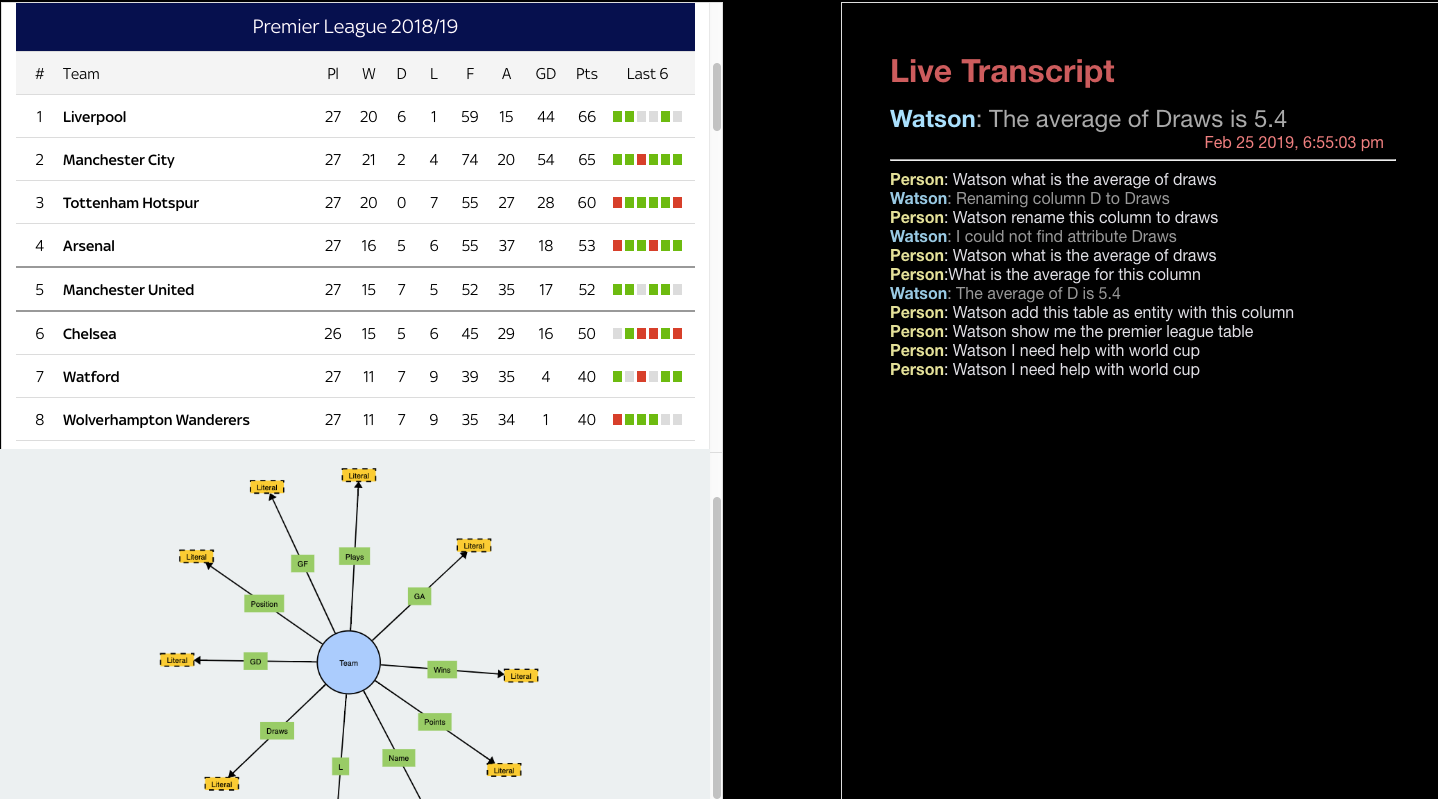
\includegraphics[width=0.8\textwidth]{chapters/03_reagent/figures/use_case_1.png}
\caption{Display of system after adding Team entity.}
\label{fig:reagent_use_case_1}
\end{figure*}

To start with, we open a page from SkySports that shows the current standings
of all teams in the football premier league~\cite{skysports_table}. To begin building
our ontology, the user can point at the displayed table and then state ``Add this table
as entity {\em team}'' or alternatively point at the column marked ``Team'' and say ``Add this
table as entity using this column''. The executor will contact \textit{Reagent} to get the columns
of the table under question. From there, the executor will send the list of columns, as well
as the entity name to our ontology as a simple JSON object, which in then converted by an
ontology pipeline into the appropriate OWL RDF structure to be stored, marking the entity as a 
Class and the columns as Object Properties linked to the class, and pointing at concrete 
Literals. After this step is completed, all entries in the table are then saved as instances
for that Class, ready to be queried. Additionally, anytime a user comes back to this page,
or a page that has a table of nearly identical structure, the system will automatically infer that the table
is of the Team class, along with automatically transforming any abbreviated columns to known
attributes if possible. Either before or after adding an entity to the ontology, a user can always go and
fill in the gaps as necessary in the system's understanding of the columns. For example, in the case of 
SkySports, while the first 4 columns have a title tag (displayed when hovering over the abbreviation), 
the rest do not and so the system saves them only as abbreviations (e.g. ``D'', ``L'', etc.). 
Additionally, while we can query the system for values of the fully named attributes, we cannot at this
time get anything for the abbreviations for what they stand for. For example, if the user
tries to ask ``What is the average of draws'', the system will respond with 
``I could not find the attribute draws''. To remedy this, the user can point at one of these
columns and then issue a new name for the column. For example, to update the
label marked ``D'', the user would point at the column and say ``Rename this column
name to Draws'', which gets automatically mirrored to our
ontology. Following this, the user can then repeat a request for the
average of draws and the system will now successfully respond with ``The average of Draws is 5.4''. The result of this sequence is shown in Figure~\ref{fig:reagent_use_case_1}, wherein we still have several more attributes that
have to be renamed due to lacking the title tag, using a similar command as
above.

After being satisfied with the constructed ``Team'' entity, the user may want
to then look at the players of one of these teams. To
do this, we open a page of a team (e.g. Manchester United) from ESPN~\cite{espn_squad_table}. When we open
the page, the system scans the table, sees if the table matches
any saved entity, which is just ``Team'' at this time and as the columns does not match the ``Team'' entity's attributes,
the system states ``I do not recognize this entity. Please add it''. Similar
to the previous entity, the user
can save the table as a new entity by first pointing at it and then saying ``Add this table as entity 'player''', which
adds a new entity ``Player'' to our ontology along with all of the columns in the
table in the same process as before. A new Player entity then appears
alongside the Team entity in the Ontology Viewer of the display, which
is shown in Figure~\ref{fig:reagent_use_case_2}.

In this case, all of the terms have title tags and so are all properly labeled when they were added, so the user does not have to do any further renaming. The user can
now query the system about these saved attributes, such as pointing at the first
row in the table and asking ``How many appearances does the player have'' which
the system responds with ``The player has 24 appearances''.

\begin{figure*}[hbtp]
\centering
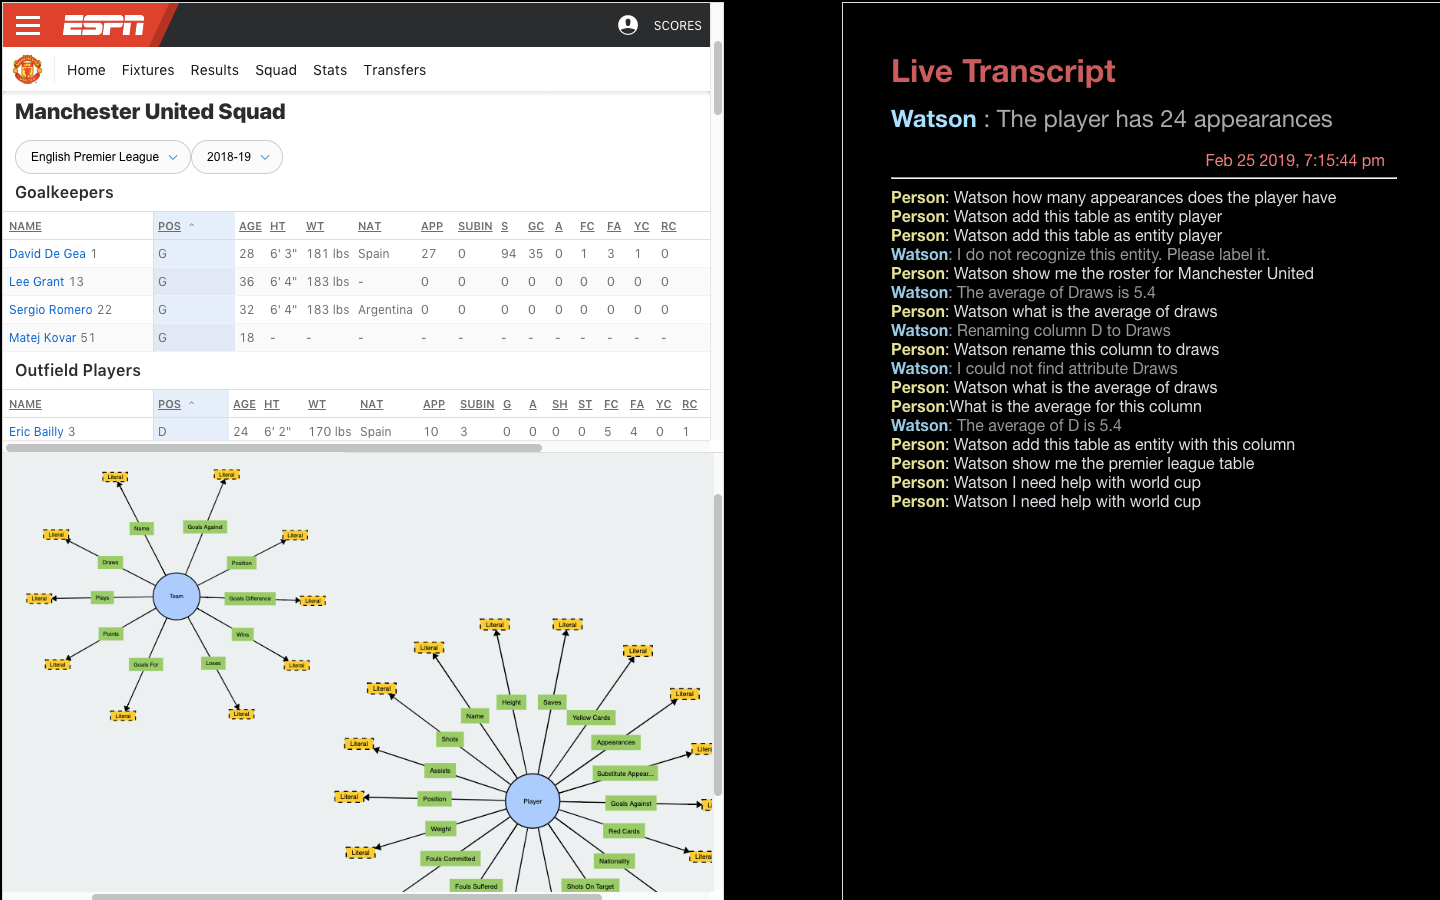
\includegraphics[width=0.8\textwidth]{chapters/03_reagent/figures/use_case_2.png}
\caption{Display of system after adding the Player entity}
\label{fig:reagent_use_case_2}
\end{figure*}

To complete our basic ontology, the user can now add a relationship
between the two saved entities. To do this, the user can simply issue
the query ``Add relationship part of between entity team and player''. The
system then adds a new Object Property link between the two marked as 
``partOf'', as shown in Figure~\ref{fig:reagent_use_case_3}. Through this connection,
the user can now start issuing queries that utilize information from both of the opened tables. For example,
the user can ask ``How many wins does the team of this player have?'' while pointing
at the player table. The system will look up who that player's team is, cross-reference it
back to the prior table, and extract the requested information, outputting it to the user.

\begin{figure*}[hbtp]
\centering
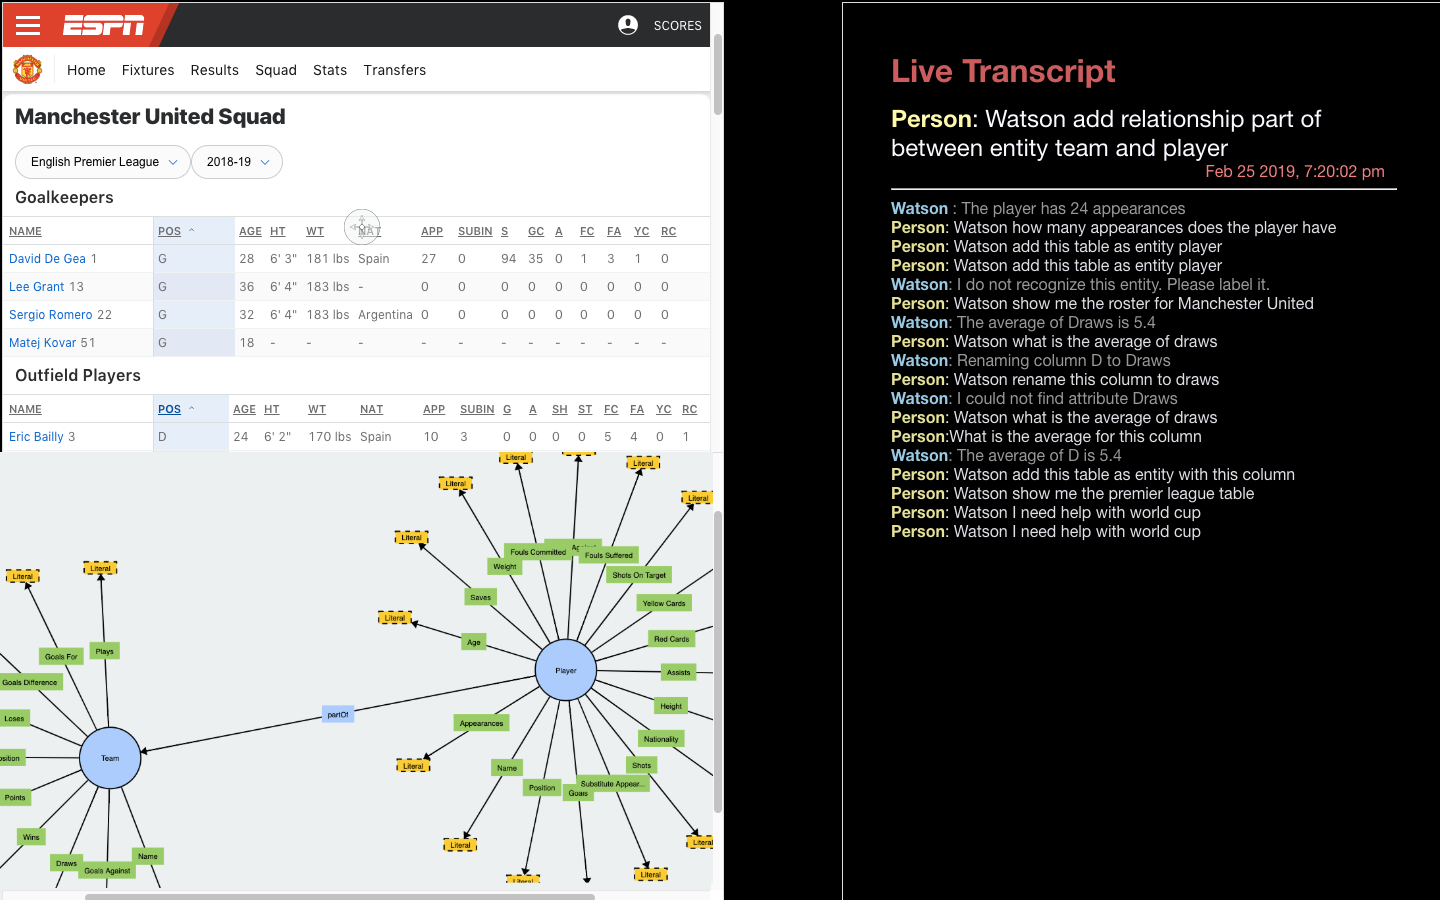
\includegraphics[width=0.8\textwidth]{chapters/03_reagent/figures/use_case_3.png}
\caption{Display of the system with the final ontology.}
\label{fig:reagent_use_case_3}
\end{figure*}

After building this ontology, whenever a user goes to a page that contains
similar content, the system will, as before, attempt to determine if the
content is of a known entity based on the table's columns, even if
the table has more or fewer attributes than have been seen. If a table is seen
with more attributes than saved in our ontology, it will ask the user if they
wish to add the attributes to the saved entity.


\section{Experiment}

To assess Reagent's ability to support natural interactions between users and third-party web pages that are typically encountered in the wild, we conducted an experiment involving nearly 200 web pages. We briefly describe the experimental setup and data collection, and then present the experimental results.

\subsection{Experimental Setup and Data Collection}
In order to obtain a collection of popular websites that contain data in tabular form, we used the Alexa service~\cite{noauthor_top_nodate}, which provides a list of the top sites viewed per month. From that service, we chose the top 10 sites in the ``Sports'' and ``Business'' categories, and filtered out those sites that contained only articles or pictures about the subject material. We crawled each of the remaining websites to generate a list of candidate pages that each contained at least one data table. In some cases, sites contained clusters of pages that were structurally identical but contained different content. For example, each team in the English Football League may have pages containing structurally identical tables, but of course the content is particular to each team. In this case, we randomly select a single representative from that cluster so as not to bias our statistics.

We then measure for each site the following quantities:
\begin{itemize}
    \item {\bf Pages.} Number of pages analyzed for the site.
    \item {\bf Tables.} Number of tables found among the pages analyzed for the site. Only the first table on each page is analyzed further.
    \item {\bf Failed.} Number of pages that Reagent was unable to parse within a timeout period of 15 seconds. For most pages, parsing takes 1-2 seconds, but for SPA type sites (where the body content dynamically loads after the rest of the page) it can take about another 2-4 seconds. Depending on how content (including ads) is loaded, a few pages take much longer because Reagent re-starts parsing whenever the page content changes.
    \item {\bf Columns.} Total number of columns among the tables analyzed for a site.
    \item {\bf Verbatim (V).} Among the columns analyzed for a site, the number for which the visible column headings are directly understandable.
    \item {\bf Interpretable (I).} Among the columns analyzed for a site, the number that, while not directly understandable, are interpretable through the use of tooltips or other metadata contained within the web page, possibly assisted by WordNet.
    \item {\bf Non-interpretable (NI).} Among the columns analyzed for a site, the number for which Reagent is unable to associate a human-understandable term, and which must therefore be defined by the user.
    \item {\bf Verbatim-Strict.} Among the tables analyzed for a site, the number for which {\em all} visible column headings are directly understandable.
    \item {\bf Interpretable-Strict.} Among the tables analyzed for a site, the number containing at least one {\bf interpretable} column.
    \item {\bf Non-interpretable-Strict.} Among the tables analyzed for a site, the number for which Reagent is unable to associate a human-understandable term for at least one column.
    \item {\bf Success Rate}. The percentage of column headers at a given site that can be interpreted correctly by Reagent, either verbatim or by using auxiliary information.
\end{itemize}

\begin{table*}[hbtp]
\centering
\begin{tabular}{ |c|c|c|c|c|c|c| }
 \hline
 Site & Pages & Failed & Cols & V & I & NI \\
 \hline
 ESPN & 93 & 19 & 1184 & 199 & 623 & 362 \\
% # of Pages: 93
% # of Pages Failed: 19
% # of Columns: 1184
% .  # abbreviated: 985
% .  # abbreviated, could expand: 623
% .  # not abbreviated: 199
% # of Tables: 196
% .  # of Tables with abbreviations: 132
% .  # of Tables with abbreviations with titles: 39
 \hline
 CricBuzz & 3 & 0 & 63 & 30 & 26 & 7\\
% # of Pages: 3
% # of Pages Failed: 0
% # of Columns: 63
% .  # abbreviated: 33
% .  # abbreviated, could expand: 26
% .  # not abbreviated: 30
% # of Tables: 5
% .  # of Tables with abbreviations: 4
% .  # of Tables with abbreviations with titles: 3
 \hline
 SkySports & 9 & 1 & 86 & 17 & 43 & 26 \\
% # of Pages: 9
% # of Pages Failed: 1
% # of Columns: 86
% .  # abbreviated: 69
% .  # abbreviated, could expand: 43
% .  # not abbreviated: 17
% # of Tables: 14
%    # of Tables with abbreviations: 13
% .  # of Tables with abbreviations with titles: 9
 \hline
 ESPN CricInfo & 6 & 0 & 73 & 9 & 56 & 8 \\
% # of Pages: 6
% # of Pages Failed: 0
% # of Columns: 73
% .  # abbreviated: 64
% .  # abbreviated, could expand: 56
% .  # not abbreviated: 9
% # of Tables: 8
% .  # of Tables with abbreviations: 7
% .  # of Tables with abbreviations with titles: 6
 \hline
 Yahoo Sports & 47 & 5 & 2171 & 719 & 1354 & 98 \\
% # of Pages: 47
% # of Pages Failed: 5
% # of Columns: 2171
% .  # abbreviated: 1452
% .  # abbreviated, could expand: 1354
% .  # not abbreviated: 719
% # of Tables: 149
% .  # of Tables with abbreviations: 121
% .  # of Tables with abbreviations with titles: 110

 \hline
 NBA.com & 7 & 0 & 263 & 40 & 0 & 223 \\
% # of Pages: 7
% # of Pages Failed: 0
% # of Columns: 263
% .  # abbreviated: 223
% .  # abbreviated, could expand: 0
% .  # not abbreviated: 40
% # of Tables: 21
% .  # of Tables with abbreviations: 11
% .  # of Tables with abbreviations with titles: 0
 \hline
 Yahoo Finance & 11 & 2 & 82 & 72 & 0 & 10 \\
% # of Pages: 11
% # of Pages Failed: 2
% # of Columns: 82
% .  # abbreviated: 10
% .  # abbreviated, could expand: 0
% .  # not abbreviated: 72
% # of Tables: 14
% .  # of Tables with abbreviations: 6
% .  # of Tables with abbreviations with titles: 0
 \hline
 BusinessInsider & 6 & 3 & 50 & 30 & 4 & 16 \\
% # of Pages: 6
% # of Pages Failed: 3
% # of Columns: 50
% .  # abbreviated: 20
% .  # abbreviated, could expand: 4
% .  # not abbreviated: 30
% # of Tables: 7
% .  # of Tables with abbreviations: 3
% .  # of Tables with abbreviations with titles: 2
 \hline
 MarketWatch & 2 & 0 & 39 & 22 & 0 & 17 \\
 % # of Pages: 2
% # of Pages Failed: 0
% # of Columns: 39
% .  # abbreviated: 17
% .  # abbreviated, could expand: 0
% .  # not abbreviated: 22
% # of Tables: 7
% .  # of Tables with abbreviations: 6
% .  # of Tables with abbreviations with titles: 0
 \hline
 {\bf Total} & {\bf 184} & {\bf 30} & {\bf 4011} & {\bf 1138} & {\bf 2106} & {\bf 767} \\
 \hline
\end{tabular}
\begin{tabular}{ |c|c|c|c|c|c| }
 \hline
 Site & Tables & V-Strict & I-Strict & NI-Strict & Success(\%)\\
 \hline
 ESPN & 196 & 64 & 39 & 93 & 69.4 \\
 \hline
 CricBuzz & 5 & 1 & 3 & 1 & 88.8\\
 \hline
 SkySports & 14 & 1 & 9 & 4 & 83.7 \\
 \hline
 ESPN CricInfo & 8 & 1 & 6 & 1 & 89.0 \\
 \hline
 Yahoo Sports & 149 & 28 & 110 & 11 & 95.5\\
 \hline
 NBA.com & 21 & 10 & 0 & 11 & 15.2 \\
 \hline
 Yahoo Finance & 14 & 8 & 0 & 6 & 87.8 \\
 \hline
 BusinessInsider & 7 & 4 & 2 & 1 & 68.0\\
 \hline
 MarketWatch & 7 & 1 & 0 & 6 & 56.4 \\
 \hline
 {\bf Total} & {\bf 421} & {\bf 118} & {\bf 169} & {\bf 134} & {\bf 80.9}\\
 \hline
\end{tabular}
\caption{Experimental Results for 9 sites with 184 pages containing tables. See above for definitions of column headings. V = Verbatim, I = Interpretable, NI = Non-interpretable.}
\label{table:sites}
\end{table*}

\subsection{Results}

The process described above yielded 184 web pages across 9 sites.
The results are summarized in  Table~\ref{table:sites}.

Across all sites, Reagent was able to successfully handle 80.9\% of all column headers. For several of the sites,
the success rates were well above 80\%, ranging up to over 95\% for Yahoo Sports.
However, for certain sites such as NBA.com, the success rate was much lower due to the absence of any
tooltip information. If we judge Reagent by the stricter criterion whereby {\em all} column headers must be
recognized automatically with no user assistance whatsoever, the overall success rate drops to
$(118 + 169) / 421 = 68.2\%$, which we feel is still quite good. These results demonstrate the general power of
Reagent and its ability to generalize across unrelated websites.

Further detailed analysis of failures and several individual cases allows us to make some additional useful observations:
\begin{enumerate}
    \item Parse failures are typically due to sites not employing an appropriate DOM structure for the table. For example, some tables do not use the conventional ``$<$th$>$'' tag for table headers, but instead use CSS classes to structure the table. Among tables that use this technique, some conventions appear to have emerged, such as using the ``colhead'' class to designate a header row -- a convention that we can exploit in future generations of Reagent.
    \item Some sites, like ESPN, constantly load content and alter its DOM over our 15 second timeout window. Currently, we rescan the entire page on a content page, but future iterations of Reagent can be made to analyze the mutation of the page, to better determine if a re-scan is actually necessary, which will prevent it from constantly re-scanning the page until the timeout, and never actually parsing the content that's shown.
    \item Many abbreviations are commonly used across different sites. For example, for all of the sports sites that we analyzed, the weight and height of a player are denoted by the abbreviations ``WT'' and ``HT''. In future generations of Reagent, we can take advantage of this fact to build a cross-site abbreviation vocabulary that can be used to infer the meaning of an abbreviation even when the web page itself provides no interpretable information.
\end{enumerate}

\section{Summary}

In this chapter, we have explained and demonstrated the Reagent system. Reagent
is capable of taking advantage of commonly-occurring structural motifs and
human-friendly tagging such as tooltips. This in-turn makes it easier for
developers to create cognitive application that support natural voice-based
interactions with pre-existing webpages containing structured data such as tables
and plots. Backing from this, we also show how Reagent can be used to help
drive a virtual mouse interface that through how it functions can be fully multi-user
through pointing and gestures, improving upon limitations of prior work. This interface
is intended to allow hooking up to a wide range of technologies demonstrated in
the prior work, including Kinect cameras~\cite{allen_rensselaer_2019},
Oblong wands~\cite{kephart_embodied_2019}, and HTC Vive controllers~\cite{zhao_immersive_2018},
as well as for allowing us to explore additional types of input mechanisms, like the
MUIFOLD system covered in the following chapter.

To demonstrate Reagent, we used it to build an ontology in OWL through two unrelated websites,
as well as provide an experimental section to showcase how the system handles
parsing of several popular websites showcasing generalizability. As part of this demonstration,
we showed how Reagent can readily learn the vocabulary of a domain by asking questions when it
does not understand the user's or the webpage's terminology. From this, we note some limitations
of our system as it applies to pages that have poor accessibility or are constantly altering
their page's content in such a way as to cause Reagent to time-out in attempting to understand
the page. Utilizing technologies of ad-blocking may be useful here, as well as for
introducing the capacity of Reagent to completely ignore portions of the page that are constantly
changing, but deemed unimportant. Additionally, one fundamental limitation of our approach is
in handling sites with iframes. Capturing interactions within iframes is not possible due to
security measures put in place by the chromium engine on Electron. Overcoming them is not
particularly feasible, but in practice iframes are not utilized heavily and so we do not view
this as a major deterrent for deploying Reagent.

An future avenue of interest would be in utilization of this technology in ontology building.
For this work, we assumed that we were starting on a blank slate. In a real-world application,
one could assume that there may be a pre-existing ontology, or that it would be possible to
import a relevant one to the domain in question. To accomplish this, we might consider utilization
of platforms such as DBPedia~\cite{auer_dbpedia_2007} or ConceptRDF~\cite{najmi_conceptrdf_2016}, both
of which readily translate into OWL. Through these, we could pre-populate an ontology with
entities and some attributes and as a user browses pages, the system could automatically, or
ask the user first, append to the imported entities building a larger and more comprehensive super-set.
